\documentclass{article}

\usepackage{graphicx}
\usepackage{xcolor}
\RequirePackage[margin=1in]{geometry}

\newcommand\todo[1]{\textcolor{red}{TODO: #1}}

\begin{document}
	
\title{Hillshade Video Script}
\author{Nathan Stouffer}
\date{}
\maketitle

\section{Intro}

\subsection{Motivation}

What I'm showing you right now is a map.
But you probably didn't need to be told that.
In fact, I would be willing to bet that you not only recognized this as a map, you also instantly discerned many topographic features about this region.
You probably recognized that this particular spot is relatively flat and that this other area is pretty steep.
Or that this is a small gully and this is a ridgeline.
Or that this face is pretty rugged while this slope is not quite as technical.

You are able to get all that complex information just from a pretty simple grayscale image.
But what's interesting, is that I bet you can't say precisely \textit{why} you are able to discern those features.
You just know it to be true.

\todo{Be more precise in this intro -- it is likely that the viewer is able to say why they know those features exist, but the point is that they can't give a precise explanation as to why. although even that doesn't cover it -- maybe it would be better to just ask the question ``What is your brain doing?'' instead of postulating that the viewer can't articulate something. It is probably better to ask, how could the viewer build something like this. Assume that they are able to explain that because of the texture of the shading, they know something to be true. But how could they produce it? I think that will be a more effective way of drawing the audience in.}

\begin{center}
	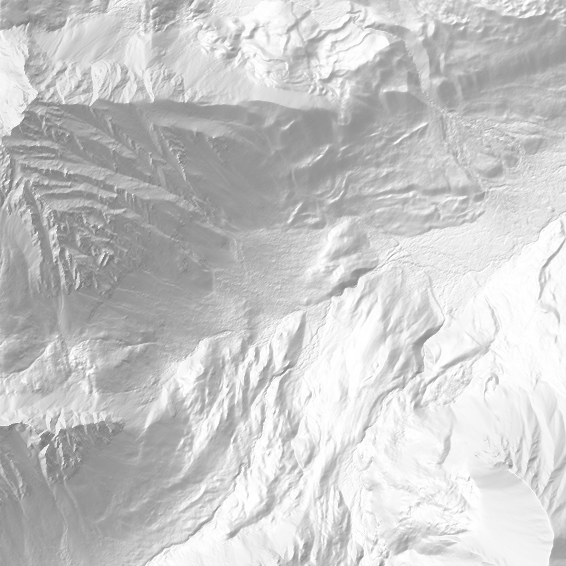
\includegraphics[width=0.5\textwidth]{assets/hillshade-example.png}
\end{center}

\subsection{Background}

\todo{Figure out some transition to this}
What's more, this isn't even a 3-dimensional map.
And I don't just mean that the screen you're viewing is 2-dimensional.
I mean that the actual model that I am rendering is 2D -- I am merely tricking your brain into thinking it is 3D.

\todo{come up with examples of directional lighting}

\section{Directional Lighting}

\subsection{Light Direction}

\subsection{Surface Normal}

\subsection{Cosine}

\subsection{Law of Cosines $=>$ Dot Product}

\section{Hillshade}

Hillshading isn't just one thing.
It is actually a term for a family of effects that can be applied to a map.
We now have the mathematical tools to build towards a very version of hillshading, but there are lots of additional techniques out there.

\section{Footnotes}

\subsection{Pseudoscopic Illusion}

\subsection{Multiple Lights}

Possibly mention Eduard Imhof.
	
\end{document}